\documentclass[a5paper, 10pt]{article}

% Текст
\usepackage[utf8]{inputenc} % UTF-8 кодировка
\usepackage[russian]{babel} % Русский язык
\usepackage{indentfirst} % красная строка в первом параграфе в главе
% Отображение страниц
\usepackage{geometry} % размеры листа и отступов
\usepackage{listings}
\usepackage{color}

\geometry{
	left=12mm,
	top=25mm,
	right=15mm,
	bottom=17mm,
	marginparsep=0mm,
	marginparwidth=0mm,
	headheight=10mm,
	headsep=7mm,
	nofoot}
\usepackage{afterpage,fancyhdr} % настройка колонтитулов
\pagestyle{fancy}
\fancypagestyle{style}{ % создание нового стиля style
	\fancyhf{} % очистка колонтитулов
	\fancyhead[LO, RE]{Лаб. работа № 4 } % название документа наверху
	\fancyhead[RO, LE]{Точностные свойства системы, астатизмы и регуляторы} % название section наверху
	\fancyfoot[RO, LE]{\thepage} % номер страницы справа внизу на нечетных и слева внизу на четных
	\renewcommand{\headrulewidth}{0.25pt} % толщина линии сверху
	\renewcommand{\footrulewidth}{0pt} % толцина линии снизу
}
\fancypagestyle{plain}{ % создание нового стиля plain -- полностью пустого
	\fancyhf{}
	\renewcommand{\headrulewidth}{0pt}
}
\fancypagestyle{title}{ % создание нового стиля title -- для титульной страницы
	\fancyhf{}
	\fancyhead[C]{{\footnotesize
			Министерство образования и науки Российской Федерации\\
			Федеральное государственное автономное образовательное учреждение высшего образования
	}}
	\fancyfoot[C]{{\large 
			Санкт-Петербург \\2024
	}}
	\renewcommand{\headrulewidth}{0pt}
}

% Математика
\usepackage{amsmath, amsfonts, amssymb, amsthm} % Набор пакетов для математических текстов
%\usepackage{dmvnbase} % мехматовский пакет latex-сокращений
\usepackage{cancel} % зачеркивание для сокращений
% Рисунки и фигуры
\usepackage[pdftex]{graphicx} % вставка рисунков
\usepackage{wrapfig, subcaption} % вставка фигур, обтекая текст
\usepackage{caption} % для настройки подписей
\captionsetup{figurewithin=none,labelsep=period, font={small,it}} % настройка подписей к рисункам
% Рисование
\usepackage{tikz} % рисование
\usepackage{circuitikz}
\usepackage{pgfplots} % графики
% Таблицы
\usepackage{multirow} % объединение строк
\usepackage{multicol} % объединение столбцов
% Остальное
\usepackage[unicode, pdftex]{hyperref} % гиперссылки
\usepackage{enumitem} % нормальное оформление списков
\setlist{itemsep=0.15cm,topsep=0.15cm,parsep=1pt} % настройки списков
% Теоремы, леммы, определения...
\theoremstyle{definition}
\newtheorem{Def}{Определение}
\newtheorem*{Axiom}{Аксиома}
\theoremstyle{plain}
\newtheorem{Th}{Теорема}
\newtheorem{Lem}{Лемма}
\newtheorem{Cor}{Следствие}
\newtheorem{Ex}{Пример}
\theoremstyle{remark}
\newtheorem*{Note}{Замечание}
\newtheorem*{Solution}{Решение}
\newtheorem*{Proof}{Доказательство}
% Свои команды
\newcommand{\comb}[1]{\left[\hspace{-4pt}\begin{array}{l}#1\end{array}\right.\hspace{-5pt} } % совокупность уравнений
% Титульный лист
\usepackage{csvsimple-l3}
\newcommand*{\titlePage}{
	\thispagestyle{title}
	\begingroup
	\begin{center}
		%		{\footnotesize
			%			Министерство образования и науки Российской Федерации\\
			%			Федеральное государственное автономное образовательное учреждение высшего образования
			%		}
		%		
		\vspace*{6ex}
		
		{\small
			САНКТ-ПЕТЕРБУРГСКИЙ НАЦИОНАЛЬНЫЙ ИССЛЕДОВАТЕЛЬСКИЙ УНИВЕРСИТЕТ ИТМО	
		}
		
		\vspace*{2ex}
		
		{\normalsize
			Факультет систем управления и робототехники
		}
		
		\vspace*{15ex}
		
		{\Large \bfseries 
			Лабораторная работа № 4
		}
\vspace*{2ex}
	{\Large \bfseries 
			
"Точностные свойства системы, астатизмы и регуляторы"
		}
\vspace*{2ex}
		
		{\normalsize
			по дисциплине Линенйные системы автоматического управления
		}

	\end{center}
	\vspace*{20ex}
	\begin{flushright}
		{\large 
			\underline{Студент}: гр. \textbf{R3338}\\
			\begin{flushright}
				\textbf{Нечаева А. А.}\\
			\end{flushright}
		}
		
		\vspace*{5ex}
		
		{\large 
			\underline{Преподаватель}: \textit{Перегудин Алексей Алексеевич}
		}
	\end{flushright}	
	\newpage
	\setcounter{page}{1}
	\endgroup}

\begin{document}
	\titlePage
	\pagestyle{style}
\newpage


\section{Задание. Задача стабилизации с идеальным дифференцирующим звеном}

Рассмотрим объект управления 2-го порядка, заданный дифференциальным уравнением
\begin{equation}
a_2 \ddot{y} + a_1 \dot{y} + a_0 y = u
\end{equation}

\subsection{Моделирование свободного движения разомкнутой системы}

Придумаем такие коэффициенты $a_i$, чтобы содержался хотя бы один неустойчивый полюс. Неустойчивый полюс, следовательно, требуется, чтобы действительная часть хотя бы одного из корней характеристического уравнения была положительной.\\

Запишем передаточную функцию системы
\begin{equation}
W(p) = \frac{\frac{1}{a_2}}{p^2 + \frac{a_1}{a_2}p +  \frac{a_0}{a_2}}
\end{equation}

Заметим, что при $a_2 = 1$, $a_1 = -4$, $a_0 = -5$, корни $\lambda_1 = -1$, $\lambda_2 = 5$. Действительная часть второго корня положительна, следовательно, полюс неустойчивый.\\

Запишем уравнение системы с учетом подобранных коэффициентов:
\begin{equation}
 \ddot{y} -4 \dot{y} -5 y = u
\end{equation}

Преобразования для построения схемы в \textit{Simulink}:

перепишем с применением оператора дифференцирования и выразим выходной сигнал $y$
\begin{multline}
p^2[y] - 4p[y] - 5y = u \Leftrightarrow p^2[y] = 4p[y] + 5y + u \Leftrightarrow \\ \Leftrightarrow y = \frac{1}{p^2} \left[ 4p[y] + 5y + u  \right] =
4 \frac{1}{p} [y] + 5 \frac{1}{p^2} [y] + \frac{1}{p^2} [u]
\end{multline}

Получили выражение, записанное с помощью оператора интегрирования. Схема, построеная для моделирования системы, приведена на рисунке 1.

\begin{figure}[h!]
\center{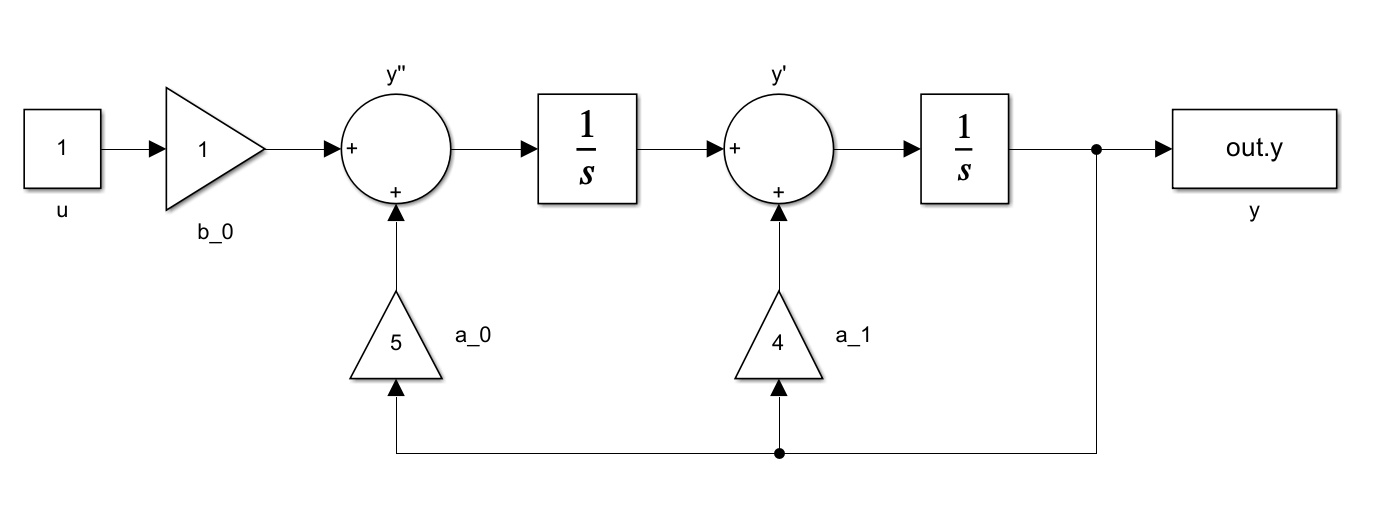
\includegraphics[width=1\linewidth]{pic/t_1_sch_1.png}}
\caption{Схема системы, построенная в \textit{Simulink}.}
\end{figure}

\newpage
Зададимся ненулевыми начальными условиями $y(0) = 1$, $\dot{y} (0) = 1$ и выполним моделирование свободного движения разомкнутой системы $y_{\text{раз}}$.

\begin{figure}[h!]
\center{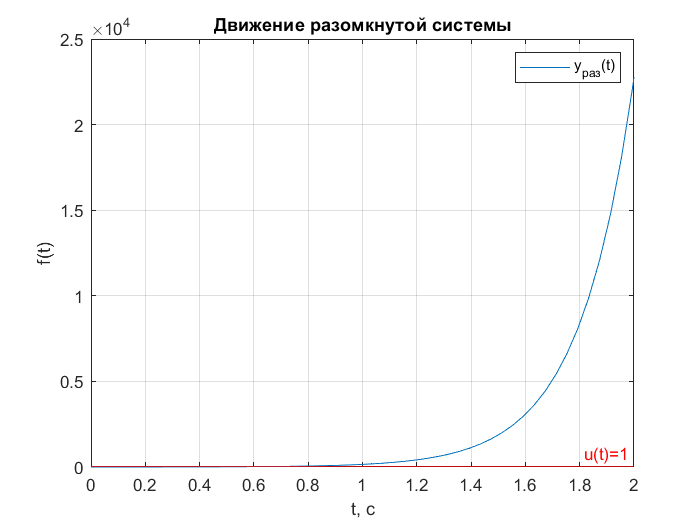
\includegraphics[width=0.9\linewidth]{pic/gr1.png}}
\caption{Результат моделирования разомкнутой системы.}
\end{figure}

\subsection{Моделирование замкнутой системы с использованием регулятора}

Рассмотрим регулятор вида
\begin{equation}
u = k_0y+ k_1 \dot{y}
\end{equation}
и построим структурную схему замкнутой системы, состоящей из объекта управления и регулятора, в режиме стабилизации (рисунок 3).

\begin{figure}[h!]
\center{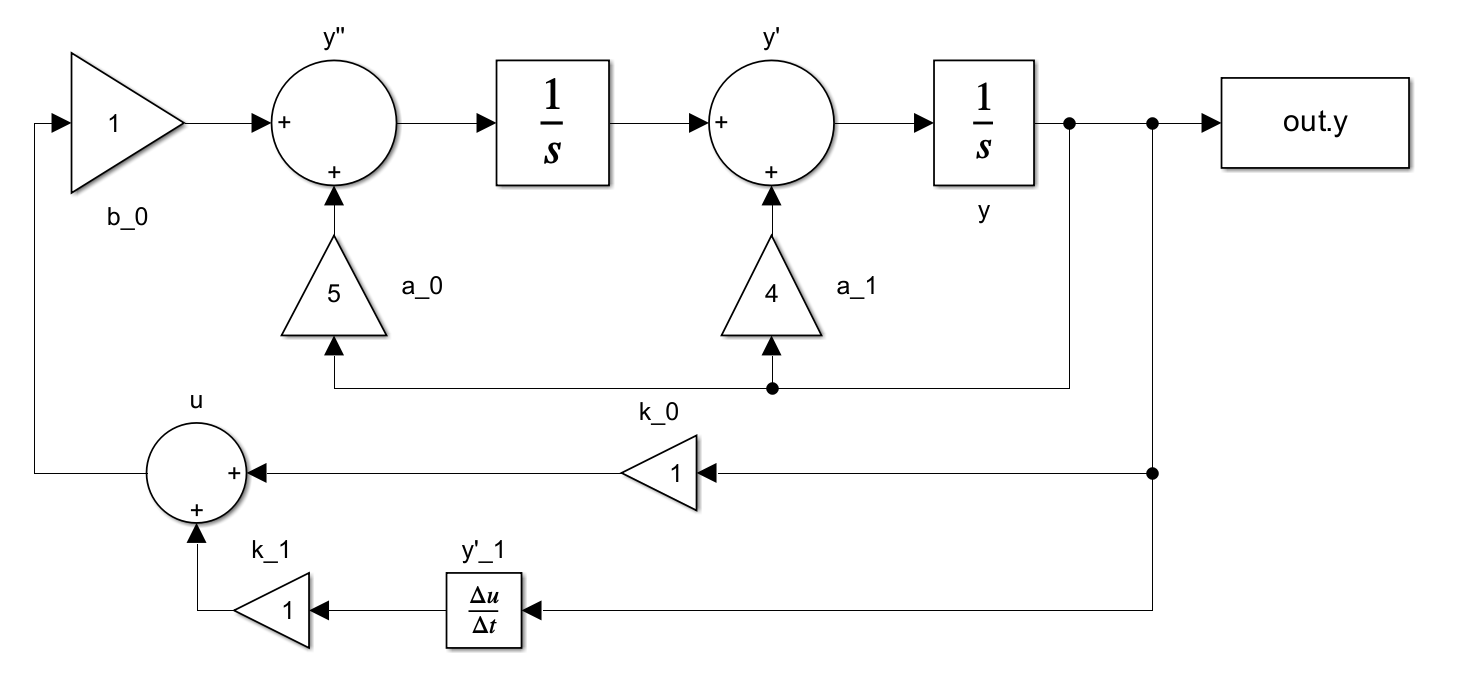
\includegraphics[width=1\linewidth]{pic/t_1_sch_2.png}}
\caption{Схема замкнутой системы, построенная в \textit{Simulink}.}
\end{figure}

Определим значения $k_i$, при которых замкнутая система будет устойчивой.
\begin{equation}
 \ddot{y} -4 \dot{y} -5 y =  k_0y+ k_1 \dot{y} \Leftrightarrow \ddot{y} - \left(4 + k_1 \right) \dot{y} -\left(5 + k_0 \right) y = 0
\end{equation}
Для системы 2-го порядка с характеристическим полиномом вида $D(\lambda) = \lambda^2 + a_1 \lambda + a_0$, согласно критерию Гурвица, необходимым и достаточным условием устойчивости является $a_i > 0$.

\begin{equation}
\begin{cases}
- \left(4 + k_1 \right) > 0\\
 -\left(5 + k_0 \right) > 0
\end{cases}
 \Leftrightarrow 
\begin{cases}
4 + k_1 < 0\\
 5 + k_0 < 0
\end{cases}
 \Leftrightarrow 
\begin{cases}
 k_1 < -4\\
 k_0 < -5
\end{cases}
\end{equation}

Зададимся значениями параметров $k_0 = -12$, $k_1 = -10$, обеспечивающим асимптотически устойчивую замкнутую систему, и выполним моделирование движения замкнутой системы $y_{\text{зам}}$ с начальными, выбранными в рамках предыдущего моделирования.

\begin{figure}[h!]
\center{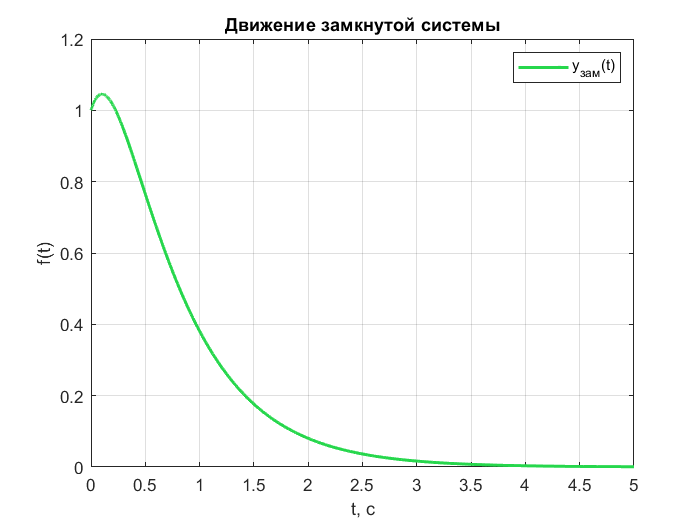
\includegraphics[width=0.9\linewidth]{pic/gr1_2.png}}
\caption{Результат моделирования замкнутой системы.}
\end{figure}

\subsection{Выводы}
В ходе выполнения задания удалось стабилизировать движение системы с помощью ПД-регулятора. График движения разомкнутой системы (рисунок 2) стремительно уходил к бесконечности с течением времени. После замыкания системы с помощью ПД-регулятора в режиме стабилизации и подбора его коэффициентов для обеспечения устойчивости системы было проведено повторное моделирование движения системы с теми же начальными условиями. В результате график движения системы стремится к нулю. Обеспечена асимптотическая устойчивость системы.

\newpage







\end{document}













